\section{MX Protocol} \label{sec:mx_protocol}
Nodes in the network need to speak the same language for efficient discovery and communication of data. Hence the following message exchange scheme (see \figref{fig:mx}) is proposed similar to \cite{Protocol_Spec}. Note that the exact mapping between the following messages and underlying transport protocol is not discussed here and may change depending on the final transport protocol chosen (\textsf{QUIC} vs \textsf{TCP})
\newline
\newline
\textbf{PUT}:  A \textsf{PUT} message contains the query to be run, an optional list of nodes to run the query against and an optional max number of hops (needed in case of an empty node list). This is used for creating or updating data in the system.
\newline
\newline
\textbf{GET}: A \textsf{GET} message contains the query to be run, max number of hops, the number of results to retrieve, the mode of retrieval (pull vs push) and a transaction identifier. Client sends this to a server to retrieve results that match the query. Parameters in \textsf{GET} can be varied depending on application needs - a streaming application may choose the push mode in which server pushes data to the client as it becomes available up until the specified number is met. A latency sensitive application may choose to retrieve a small number of results in a batch in one pull.
\newline
\newline
\textbf{SEND}: Servers respond to each \textsf{GET} message with one or more \textsf{SEND} messages with results. In pull mode, there is only one \textsf{SEND} message followed by an \textsf{END} message where as in push mode there are multiple \textsf{SEND} messages followed by an \textsf{END} message.
\newline
\newline
\textbf{END}: Servers send \textsf{END} messages to clients to indicate that they have finished sending all results in response to a particular \textsf{GET} message.
\newline
\newline
\textbf{CLOSE}: A client can send a \textsf{CLOSE} message to the server to indicate that it no longer is interested in the remaining query results and close the transaction. It doesn't have to wait until all the results are retrieved.
\newline
\newline
\textbf{OK}: Server sends this message to a client as a positive acknowledgment to a client's message.
\newline
\newline
\textbf{ERROR}: Server sends this message to a client as a negative acknowledgment to a client's message.
\begin{figure}[h!] \centering
	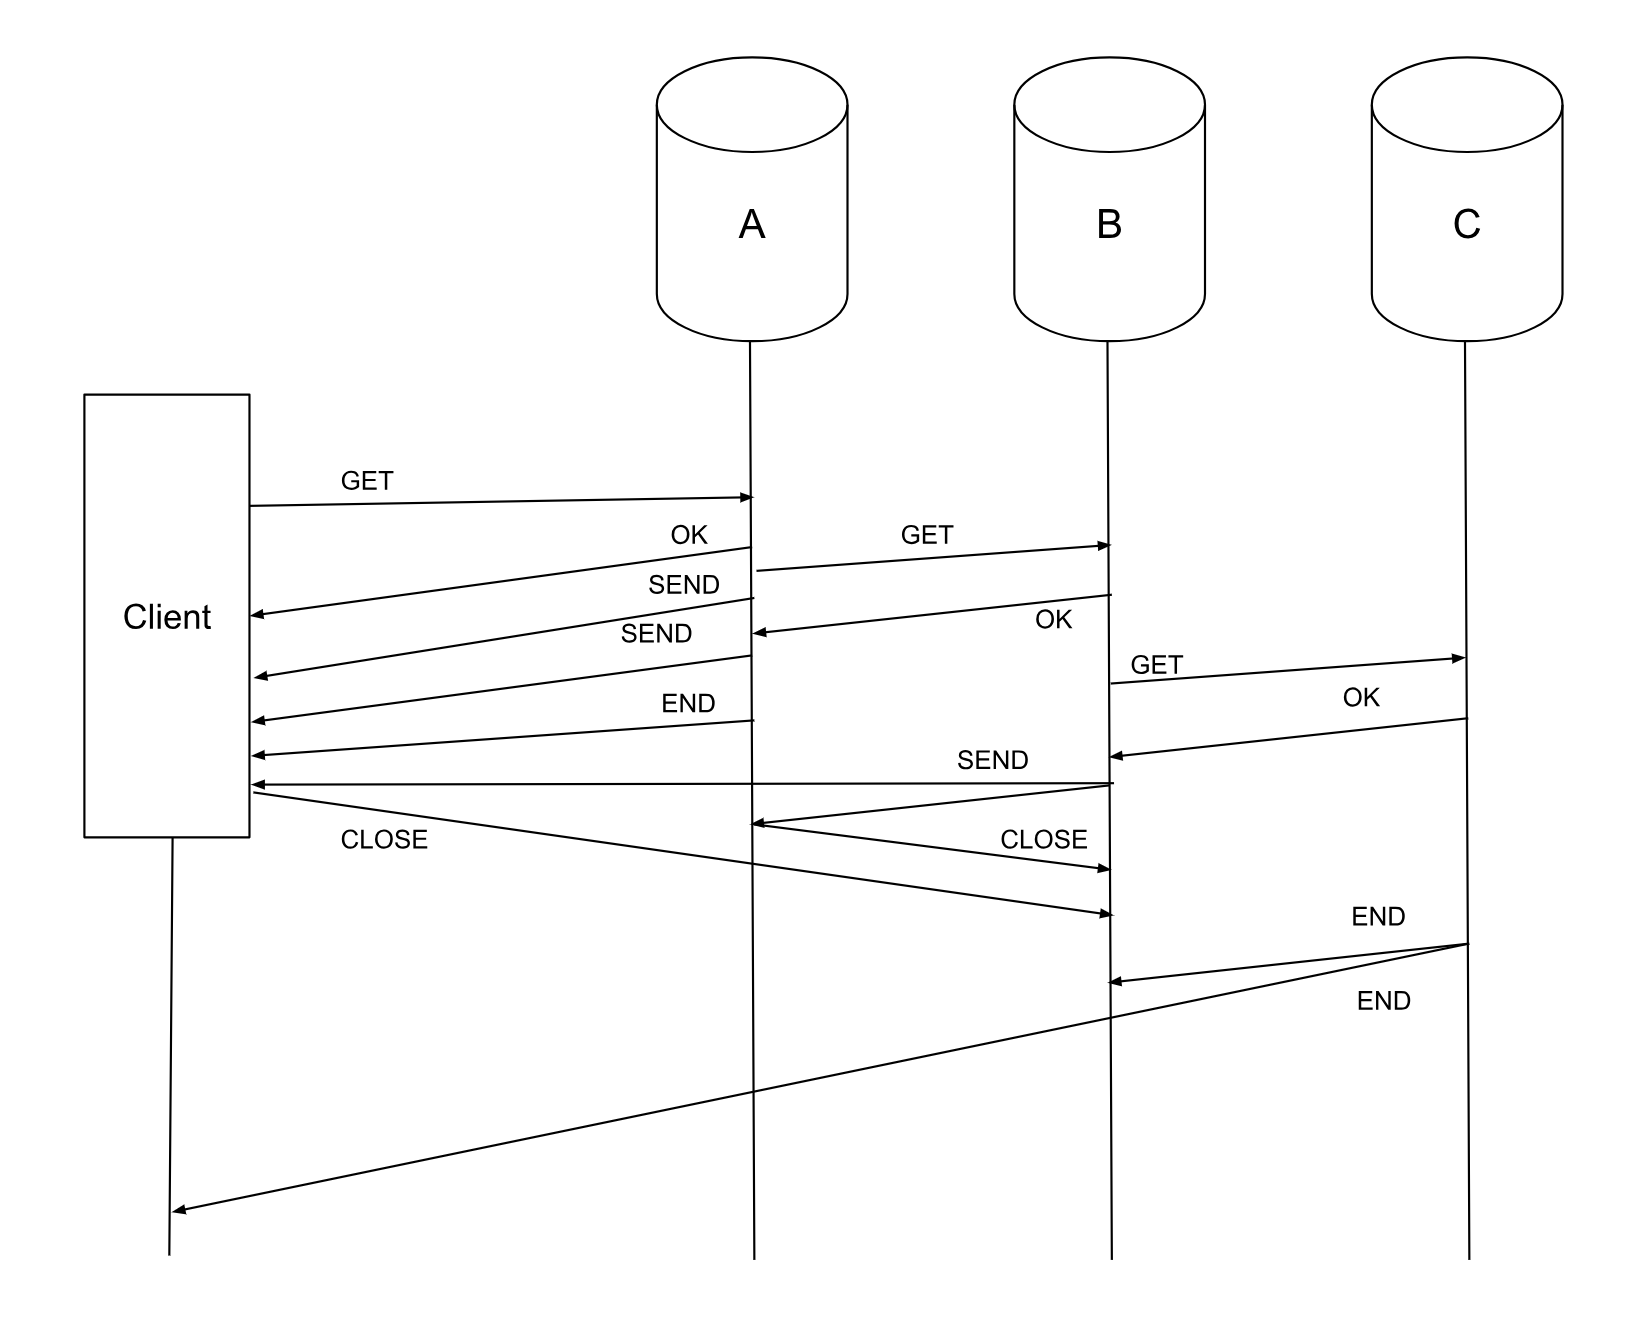
\includegraphics[width=\fscale{0.76}]{mx1.png}
	\caption{\textsf{GET} message flow, time increasing from top to bottom}
	\label{fig:mx}
\end{figure}


